\ifx\wholebook\relax \else
% ------------------------

\documentclass[b5paper]{ctexart}
\usepackage[nomarginpar
  %, margin=.5in
]{geometry}

\addtolength{\oddsidemargin}{-0.05in}
\addtolength{\evensidemargin}{-0.05in}
\addtolength{\textwidth}{0.1in}

\usepackage[cn]{../../../prelude}

\setcounter{page}{1}

\begin{document}

\title{基数树}

\author{刘新宇
\thanks{{\bfseries 刘新宇 } \newline
  Email: liuxinyu95@gmail.com \newline}
  }

\maketitle
\fi

\markboth{基数树}{基本算法}

\ifx\wholebook\relax
\chapter{基数树}
\numberwithin{Exercise}{chapter}
\fi

%\section{简介}
\label{introduction} \index{基数树}

排序二叉树将信息存储在节点中。我们可以用边(edge)来携带信息么?基数树(Radix tree),包括trie、前缀树、后缀树就是根据这一思路设计出的数据结构。它们产生于1960年代,被广泛用于编译器\cite{okasaki-int-map}和生物信息处理(如DNA模式匹配)\cite{wiki-suffix-tree}等领域。

\begin{figure}[htbp]
  \centering
  \includegraphics[scale=0.4]{img/radix-tree.ps}
  \caption{基数树}
  \label{fig:radix-tree}
\end{figure}

图\ref{fig:radix-tree}展示了一棵基数树。它包含了二进制串1011、10、011、100、0。如果查找二进制数$k=(b_0b_1...b_n)_2$,我们首先检查左侧的最高位$b_0$。若为0,则转向左子树继续查找;若为1,则转向右子树。接着,我们检查第二位,并重复这一过程直到处理完所有的$n$位或到达某一叶子节点。我们并不需要在节点中存储键(key),这一信息由边来代表。图\ref{fig:radix-tree}标注在节点中的键仅仅是为了示意。对于整数类型的键,我们可以使用二进制,并利用位运算进行操作。

\section{整数trie}
\label{int-trie} \index{基数树!整数trie}

我们称图\ref{fig:radix-tree}所示的数据结构为\emph{binary trie}。Trie是Edward Fredkin在1960年提出的。它来自英文单词re\textbf{trie}val。Fredkin将其读作/'tri:/,但其他人读作/'trai/(和英文单词try的发音相同)\cite{wiki-trie}。有些情况下trie也被称为前缀树,在本章中,trie和前缀树分指不同的数据结构。一棵binary trie是一种特殊的二叉树,每个键的位置由它的二进制位来决定。0表示“向左”,1表示“向右”\cite{okasaki-int-map}。考虑图\ref{fig:big-endian-trie}中的trie,3个不同串``11''、``011''、``0011''代表同一个十进制整数3。

\begin{figure}[htbp]
  \centering
  \includegraphics[scale=0.4]{img/big-endian-trie.ps}
  \caption{大端(big-endian)trie}
  \label{fig:big-endian-trie}
\end{figure}

如果把前面的0也当作有效位,在一个32位整数的系统中,向空trie插入1,结果将是一棵32层的树。为了解决这一问题,Okasaki建议使用小端整数\cite{okasaki-int-map}。二进制数的最高位(MSB)通常在左边,最低位(LSB)在右边。这种形式称为大端整数,反之最高位在右边称为小端整数。使用小端,1表示为$(1)_2$,、2表示为$(01)_2$、3表示为$(11)_2$……

\subsection{定义}
我们可以重用二叉树的定义。一个节点要么为空,要么包含左右子树和一个值(值可以为空)左子树编码为0,右子树编码为1。

\lstset{frame = single}
\begin{Haskell}
data IntTrie a = Empty
               | Branch (IntTrie a) (Maybe a) (IntTrie a)
\end{Haskell}

对于binary trie中的任一节点,其对应的整数键是由节点的位置唯一确定的。因此我们无需在节点中存储键,而只需存储值。键的类型被固定为整数,如果值的类型为$A$,则树的类型为$IntTrie\ A$。

\subsection{插入}
\index{整数trie!插入}

当插入整数键$k$和值$v$时,我们将$k$转换成二进制。如果$k$是偶数,最低位是0,我们递归向左子树插入;如果$k$是奇数,最低位是1,我们递归向右子树插入。接下来我们将$k$除以2取整以去掉最低位。对于非空的trie树$T = (l, v', r)$,其中$l$、$r$是左右子树,$v'$是值(可为空),函数$insert$的定义如下:

\be
\begin{array}{rcl}
insert\ \nil\ k\ v & = & insert (\nil, \textit{Nothing}, \nil)\ k\ v \\
insert\ (l, v', r)\ 0\ v & = & (l, \textit{Just}\ v, r) \\
insert\ (l, v', r)\ k\ v & = & \begin{cases}
  even(k): & (insert\ l\ \dfrac{k}{2}\ v, v', r) \\
  odd(k) : & (l, v', insert\ r\ \lfloor \dfrac{k}{2} \rfloor\ v) \\
\end{cases}
\end{array}
\ee

如果$k = 0$,我们将$v$存入节点。如果$T = \nil$,结果为$(\nil, \textit{Just}\ v, \nil)$。只要$k \neq 0$,我们就根据$k$的奇偶性前进,遇到$\nil$就建立一个空叶子节点$(\nil, \textit{Nothing}, \nil)$。如果$k$已经存在,这一算法覆盖以前的值。我们也可以用一个列表存储多个值,并将$v$添加到列表中。图\ref{int-trie}的例子是依次插入映射对\{$ 1 \rightarrow a, 4 \rightarrow b, 5 \rightarrow c, 9 \rightarrow d$\}的结果。下面的例子程序实现了$insert$函数:

\begin{figure}[htbp]
  \centering
  \includegraphics[scale=0.5]{img/int-trie.ps}
  \caption{用小端整数trie,包含映射:
          \{$ 1 \rightarrow a, 4 \rightarrow b, 5 \rightarrow c, 9 \rightarrow d$\}}
  \label{fig:int-trie}
\end{figure}

\begin{Haskell}
insert Empty k x = insert (Branch Empty Nothing Empty) k x
insert (Branch l v r) 0 x = Branch l (Just x) r
insert (Branch l v r) k x | even k    = Branch (insert l (k `div` 2) x) v r
                          | otherwise = Branch l v (insert r (k `div` 2) x)
\end{Haskell}

为了判定一个数的奇偶性,我们可以判断它除以2的余数(模2)是否为0:$even(k) = (k \bmod 2 = 0)$,活着使用位运算,如:\texttt{(k \& 0x1) == 0}。我们也可以消除递归用循环实现插入算法:

%\begin{algorithm}
\begin{algorithmic}[1]
\Function{Insert}{$T, k, v$}
  \If{$T =$ NIL}
    \State $T \gets$ \Call{Empty-Node}{}  \Comment{(NIL, Nothing, NIL)}
  \EndIf
  \State $p \gets T$
  \While{$k \neq 0$}
    \If{\Call{Even?}{$k$}}
      \If{\Call{Left}{$p$} = NIL}
        \State \Call{Left}{$p$} $\gets$ \Call{Empty-Node}{}
      \EndIf
      \State $p \gets$ \Call{Left}{$p$}
    \Else
      \If{\Call{Right}{$p$} = NIL}
        \State \Call{Right}{$p$} $\gets$ \Call{Empty-Node}{}
      \EndIf
      \State $p \gets$ \Call{Right}{$p$}
    \EndIf
    \State $k \gets \lfloor k/2 \rfloor$
  \EndWhile
  \State \Call{Value}{$p$} $\gets v$
  \State \Return $T$
\EndFunction
\end{algorithmic}
%\end{algorithm}

\textproc{Insert}接受3个参数:trie树$T$、要插入的键$k$和相应的数据$v$。对于有$m$二进制位的整数$k$,这一算法访问trie中的$m$层,时间复杂度为$O(m)$。

\subsection{查找}
\index{整数trie!查找}

在小端整数trie中查找数字$k$时,若树为空,则显然$k$不存在;如果$k=0$,则返回当前根节点中存储的数据。否则根据最后一位是0还是1,在左右分支进行递归查找。

\be
lookup(T, k) =  \left \{
  \begin{array}
  {r@{\quad:\quad}l}
  \phi & T = \phi \\
  d & k = 0 \\
  lookup(T_l, k / 2) & even(k) \\
  lookup(T_r, \lfloor k / 2 \rfloor) & otherwise
  \end{array}
\right.
\ee

下面的Haskell例子程序实现了递归查找算法。

\lstset{language=Haskell}
\begin{lstlisting}[style=Haskell]
search Empty k = Nothing
search t 0 = value t
search t k = if even k then search (left t) (k `div` 2)
             else search (right t) (k `div` 2)
\end{lstlisting}

也可以用命令式的方式实现查找,我们从$k$的二进制形式最右侧开始,逐位检查,如果为0,就继续在左侧分支查找;如果为1,则在右侧分支查找。直到所有位都处理完毕。

\begin{algorithmic}[1]
\Function{Lookup}{$T, k$}
  \While{$k \neq 0 \land T \neq $NIL}
    \If{ \Call{Even?}{$k$} }
      \State $T \gets$ \Call{Left}{$T$}
    \Else
      \State $T \gets$ \Call{Right}{$T$}
    \EndIf
    \State $k \gets \lfloor k/2 \rfloor$
  \EndWhile
  \If{$T \neq $ NIL}
    \State \Return \Call{Data}{$T$}
  \Else
    \State \Return not found \EndIf
\EndFunction
\end{algorithmic}

下面的Python例子程序实现了查找算法。

\lstset{language=Python}
\begin{lstlisting}
def lookup(t, key):
    while t is not None and k != 0:
        if key & 1 == 0:
            t = t.left
        else:
            t = t.right
        key = key >> 1
    return None if t is None else t.value
\end{lstlisting}

若待查找的key有$m$位,则查找算法的复杂度为$O(m)$。

% ================================================================
%               Int 前缀树
% ================================================================
\section{整数前缀树}
\label{int-patricia}
\index{整数Patricia}
\index{整数前缀树}

Trie的缺点是空间消耗大。如图\ref{int-trie}所示,只有叶子节点存储了最终的数据。整数Trie中有大量的节点只包含一棵子树。为了提高空间利用率,我们可以将一连串“独生子女”压缩成一个节点。前缀树就是这样的数据结构,由Donald R. Morrison在1968年提出。在他的论文中,前缀树被称为Patricia。是\textbf{P}ractical \textbf{A}lgorithm \textbf{T}o \textbf{R}etrieve \textbf{I}nformation \textbf{C}oded \textbf{I}n \textbf{A}lphanumeric的首字母缩写\cite{patricia-morrison}。

Okasaki给出了整数前缀树的实现\cite{okasaki-int-map}。将图\ref{fig:int-trie}中只有一个子树的节点合并后,可以得到一棵如图\ref{fig:little-endian-patricia}所示的树。

\begin{figure}[htbp]
  \centering
  \includegraphics[scale=0.5]{img/little-endian-patricia.ps}
  \caption{小端前缀树实现的映射
     \{$ 1 \rightarrow a, 4 \rightarrow b, 5 \rightarrow c, 9 \rightarrow d$\}}
  \label{fig:little-endian-patricia}
\end{figure}

观察此图,可以发现分支节点所代表的key是它的所有子分支的公共前缀。这些子分支key的开头部分一样,然后从某一点开始出现不同。和Trie相比,前缀树节省了很多空间。

和整数Trie不同,整数前缀树可以使用大端实现而不会遇到\ref{int-trie}中所描述的0前缀问题。第一位有效数字前的0全都被去除以节省空间。Okasaki在\cite{okasaki-int-map}中列出了大端前缀树的优点。

% ================================================================
%                 Definition of int 前缀树 tree
% ================================================================
\subsection{定义}

整数前缀树是一种特殊的二叉树。它或者为空,或者是一个节点。节点有两种类型:

\begin{itemize}
\item 叶子节点:包含一个整数key和相应的数据(数据可为空);
\item 分支节点:包含左右子分支。两个子分支的key具有最长的二进制公共前缀。其中左侧子分支的下一位是0,而右侧子分支的下一位是1。
\end{itemize}

下面的Haskell例子代码定义了前缀树:

\lstset{language=Haskell}
\begin{lstlisting}[style=Haskell]
type Key = Int
type Prefix = Int
type Mask = Int

data IntTree a = Empty
               | Leaf Key a
               | Branch Prefix Mask (IntTree a) (IntTree a)
\end{lstlisting}

为了表示从哪一位开始左右分支的key变得不相同,分支节点中保存了掩码信息。通常掩码是2的整数次幂,形如$2^n$,其中$n$是非负整数。所有低于$n$的二进制位都不属于key的公共前缀。

下面的Python例子代码定义了前缀树和相应的辅助函数。

\lstset{language=Python}
\begin{lstlisting}
class IntTree:
    def __init__(self, key = 0, value = None):
        self.key = key
        self.value = value
        self.prefix = key
        self.mask = 1
        self.left = self.right = None

    def isleaf(self):
        return self.left is None and self.right is None

    def replace(self, x, y):
        if self.left == x:
            self.left = y
        else:
            self.right = y

    def match(self, k):
        return maskbit(k, self.mask) == self.prefix
\end{lstlisting}

其中match判断节点的前缀在掩码前是否和给定的key一致。我们稍后介绍它的实现。

% ================================================================
%                 Insertion of int 前缀树
% ================================================================
\subsection{插入}
\index{整数前缀树!插入}
当插入key时,如果树为空,结果为一个叶子节点,key和相关的数据存储于节点中,如图\ref{fig:int-patricia-insert-a}所示。

\begin{figure}[htbp]
  \centering
    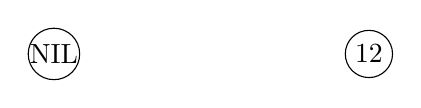
\begin{tikzpicture}[scale=1,
      treenode/.style={circle, draw, inner sep= 0pt, minimum size = .6cm}]
    \node[treenode] at (-2, 0) {NIL};
    \node[treenode] at (2, 0) {12};
    \end{tikzpicture}
  %\includegraphics[scale=0.8]{img/int-patricia-insert-a.ps}
  \caption{左侧:树为空;右侧:插入整数12后}
  \label{fig:int-patricia-insert-a}
\end{figure}

如果树只有一个叶子节点$x$,我们把待插入的key和数据放入一个新的叶子节点$y$中。然后创建一个新的分支节点,并令$x$和$y$为这一新分支节点的两个子节点。为了确定$y$应该在左边还是右边,我们需要找到$x$和$y$的最长公共前缀。举个例子,假设$key(x)$为12(二进制1100),$key(y)$为15(二进制1111),则最长公共前缀为二进制$11oo$,其中$o$代表我们不关心的二进制位,我们可以使用一个整数通过掩码来去掉这些位。在这个例子中,可以用4(二进制100)作为掩码。最长公共前缀后面的一位代表$2^1$。$key(x)$中这一位是0,而$key(y)$中这一位是1。因此$x$是左子树,而$y$是右子树。这个例子如图\ref{fig:int-patricia-insert-b}所示。

\begin{figure}[htbp]
  \centering
  \includegraphics[scale=0.7]{img/int-patricia-insert-b.ps}
  \caption{左侧:只含有一个叶子节点12的树;右侧:插入整数15后}
  \label{fig:int-patricia-insert-b}
\end{figure}

如果树既不为空,也不是一个单独的叶子节点,我们需要先比较待插入的key和根节点中记录的最长公共前缀是否一致。如果一致,则根据接下来的位是0还是1递归地在左侧或右侧进行插入。例如,若将整数14(二进制1110)插入图\ref{fig:int-patricia-insert-b}中所示的树中,由于最长公共前缀是$11oo$而接下来的一位($2^1$位)是1,所以需要将14递归插入到右子树。

最后,如果待插入的整数和根节点中记录的最长公共前缀不一致,我们需要从根节点分出一棵新的枝杈。图\ref{fig:int-patricia-insert-c}展示了这两种不同的情况。

\begin{figure}[htbp]
  \centering
  \subcaptionbox{插入整数14。它和最长公共前缀$(1100)_2$一致。需要将其递归插入到右侧分支中。}{\includegraphics[scale=0.5]{img/int-patricia-insert-c.ps}}\\
  \subcaptionbox{插入整数5。它和最长公共前缀$(1100)_2$不一致。需要新分杈出一个分支。}{\includegraphics[scale=0.5]{img/int-patricia-insert-d.ps}}
  \caption{向分支节点插入整数}
  \label{fig:int-patricia-insert-c}
\end{figure}

记要插入的整数为$k$,数据为$v$的节点为$(k, v)$,分支节点记为$(p, m, T_l, T_r)$,其中$p$代表最长公共前缀,$m$表示掩码,$T_l$和$T_r$分别代表左右子分支。上述情况可以归纳为下面的插入算法:

\be
insert(T, k, v) = \left \{
  \begin{array}
  {r@{\quad:\quad}l}
  (k, v) & T = \phi \lor T = (k, v') \\
  join(k, (k, v), k', T) & T = (k', v') \\
  (p, m, insert(T_l, k, v), T_r) & T = (p, m, T_l, T_r), match(k, p, m), zero(k, m) \\
  (p, m, T_l, insert(T_r, k, v)) & T = (p, m, T_l, T_r), match(k, p, m), \lnot zero(k, m) \\
  join(k, (k, v), p, T) & T = (p, m, T_l, T_r), \lnot match(k, p, m)
  \end{array}
\right.
\ee

第一行处理边界情况,$T$或者为空,或者是一个具有同样key的叶子节点。我们用新的值覆盖此前的数据。

第二行处理$T$为叶子节点,但是key不同的情况。这时需要分支出一个新的叶子节点,为此,我们需要计算出最长公共前缀,并判断哪个在左侧,哪个在右侧。函数$join(k_1, T_1, k_2, T_2)$负责这些处理,我们稍后会定义它。

第三、四行处理$T$为分支节点,且分支代表的前缀和待插入的整数一致的情况。如果接下来的一位是0,则第三行会递归地向左侧分支进行插入。否则第四行递归地向右侧分支插入。

最后一行处理$T$为分支节点,但是key不一致的情况。我门需要调用$join$函数来分支出一个新的叶子节点。

接下来需要定义函数$match(k, p, m)$用以判断整数$k$在掩码$m$以上的位是否和$p$一致。也就是检查$p$在掩码以上的位是否为$k$的一个前缀。例如,一个分支节点的key表示为二进制$(p_np_{n-1} ... p_i...p_0)_2$,待插入的key $k$的二进制形式为$(k_nk_{n-1} ... k_i ... k_0)_2$,掩码为$(100...0)_2=2^i$。则称$k$、$p$、$m$一致当且仅当对于任意$j$, $i \leq j \leq n$有$p_j=k_j$。

我们可以通过判断等式$mask(k, m) = p$是否成立来实现$match$函数。其中$mask(x, m) = \overline{m-1} \& x$。即先对$m-1$按位取反,然后将结果和$x$按位进行与运算。

函数$zero(k, m)$检查公共前缀接下来的一位是否为0。我们可以将掩码$m$向右做1位移位运算,接下来和$k$进行按位与运算。

\be
zero(k, m) = k \& shift_r(m, 1)
\ee

举例来说,若$m = (100...0)_2 = 2^i$、$k = (k_nk_{n-1}...k_i1...k_0)_2$,由于$k_i$的下一位是1,所以$zero(k, m)$的结果为false;反之,若$k = (k_nk_{n-1}...k_i0...k_0)_2$,则结果为true。

函数$join(p_1, T_1, p_2, T_2)$接受两个前缀和两棵树作为参数。它找出$p_1$与$p_2$的最长公共前缀,然后创建一个新的分支节点,并将$T_1$和$T_2$作为子节点。

\be
join(p_1, T_1, p_2, T_2) = \left \{
  \begin{array}
  {r@{\quad:\quad}l}
  (p, m, T_1, T_2) & zero(p1, m), (p, m) = LCP(p_1, p_2) \\
  (p, m, T_2, T_1) & \lnot zero(p1, m)
  \end{array}
\right.
\ee

为了计算$p_1$和$p_2$的最长公共前缀,我们可以先对它们计算异或,然后用这个结果的有效位数产生一个掩码$m = 2^{|xor(p_1,p_2)|}$。最长公共前缀就可以用这个掩码和$p_1$与$p_2$中的任何一个得出。例如:

\be
p = mask(p_1, m)
\ee

下面的Haskell例子程序实现了插入算法:

\begin{lstlisting}[style=Haskell]
import Data.Bits

insert t k x
   = case t of
       Empty -> Leaf k x
       Leaf k' x' -> if k==k' then Leaf k x
                     else join k (Leaf k x) k' t -- t@(Leaf k' x')
       Branch p m l r
          | match k p m -> if zero k m
                           then Branch p m (insert l k x) r
                           else Branch p m l (insert r k x)
          | otherwise -> join k (Leaf k x) p t -- t@(Branch p m l r)

join p1 t1 p2 t2 = if zero p1 m then Branch p m t1 t2
                                else Branch p m t2 t1
    where
      (p, m) = lcp p1 p2

lcp :: Prefix -> Prefix -> (Prefix, Mask)
lcp p1 p2 = (p, m) where
    m = bit (highestBit (p1 `xor` p2))
    p = mask p1 m

highestBit x = if x == 0 then 0 else 1 + highestBit (shiftR x 1)

mask x m = (x .&. complement (m-1)) -- complement表示按位取反

zero x m = x .&. (shiftR m 1) == 0

match k p m = (mask k m) == p
\end{lstlisting}

插入算法也可以用命令式方法实现:

\begin{algorithmic}[1]
\Function{Insert}{$T, k, v$}
  \If{$T = $ NIL}
    \State $T \gets$ \Call{Create-Leaf}{$k, v$}
    \State \Return $T$
  \EndIf
  \State $y \gets T$
  \State $p \gets$ NIL
  \While{$y$ is not leaf, and \textproc{Match}($k$, \Call{Prefix}{$y$}, \Call{Mask}{$y$})}
    \State $p \gets y$
    \If{\textproc{Zero?}($k$, \Call{Mask}{$y$})}
      \State $y \gets$ \Call{Left}{$y$}
    \Else
      \State $y \gets$ \Call{Right}{$y$}
    \EndIf
  \EndWhile
  \If{$y$ is leaf, and $k = $ \Call{Key}{$y$}}
    \State \Call{Data}{$y$} $\gets v$
  \Else
    \State $z \gets$ \textproc{Branch}($y$, \Call{Create-Leaf}{$k, v$})
    \If{$p = $ NIL}
      \State $T \gets z$
    \Else
      \If{\Call{Left}{$p$} $ = y$}
        \State \Call{Left}{$p$} $\gets z$
      \Else
        \State \Call{Right}{$p$} $\gets z$
      \EndIf
    \EndIf
  \EndIf
  \State \Return $T$
\EndFunction
\end{algorithmic}

函数\textproc{Branch}($T_1, T_2$)的作用和前面定义的$join$类似。它创建一个新的分支节点,计算最长公共前缀,然后将$T_1$和$T_2$设置为两棵子树。

\begin{algorithmic}[1]
\Function{Branch}{$T_1, T_2$}
  \State $T \gets$ \Call{Empty-Node}{}
  \State $($ \Call{Prefix}{$T$}, \Call{Mask}{$T$} $) \gets$ \textproc{LCP}(\Call{Prefix}{$T_1$}, \Call{Prefix}{$T_2$})
  \If{\textproc{Zero?}(\Call{Prefix}{$T_1$}, \Call{Mask}{$T$})}
    \State \Call{Left}{$T$} $\gets T_1$
    \State \Call{Right}{$T$} $\gets T_2$
  \Else
    \State \Call{Left}{$T$} $\gets T_2$
    \State \Call{Right}{$T$} $\gets T_1$
  \EndIf
  \State \Return $T$
\EndFunction
\end{algorithmic}

下面的Python例子程序实现了插入算法:

\lstset{language=Python}
\begin{lstlisting}
def insert(t, key, value):
    if t is None:
        return IntTree(key, value)
    node = t
    parent = None
    while (not node.isleaf()) and node.match(key):
        parent = node
        if zero(key, node.mask):
            node = node.left
        else:
            node = node.right
    if node.isleaf() and key == node.key:
        node.value = value
    else:
        p = branch(node, IntTree(key, value))
        if parent is None:
            return p
        parent.replace(node, p)
    return t
\end{lstlisting}

辅助函数\texttt{branch}和\texttt{lcp}等定义如下:

\begin{lstlisting}
def maskbit(x, mask):
    return x & (~(mask - 1))

def zero(x, mask):
    return x & (mask >> 1) == 0

def lcp(p1, p2):
    diff = p1 ^ p2
    mask = 1
    while diff != 0:
        diff >>= 1
        mask <<= 1
    return (maskbit(p1, mask), mask)

def branch(t1, t2):
    t = IntTree()
    (t.prefix, t.mask) = lcp(t1.prefix, t2.prefix)
    if zero(t1.prefix, t.mask):
        t.left, t.right = t1, t2
    else:
        t.left, t.right = t2, t1
    return t
\end{lstlisting}

图\ref{fig:int-patricia-haskell-insert}展示了使用插入算法构造的前缀树。

\begin{figure}[htbp]
  \centering
  \includegraphics[scale=0.6]{img/int-patricia-haskell-insert.ps}
  \caption{插入映射$1 \rightarrow x, 4 \rightarrow y, 5 \rightarrow z$到一个大端整数前缀树树}
  \label{fig:int-patricia-haskell-insert}
\end{figure}


% ================================================================
%                 Lookup in int 前缀树
% ================================================================
\subsection{查找}
\index{整数前缀树!查找}

如果前缀树为空或仅包含一个叶子节点,且节点的key不等于待查找的整数,则查找结果为空。如果树仅有一个叶子节点,且节点的key恰好等于待查找的值,则查找结果就是该叶子节点所包含的数据。否则,树$T$是一个分支节点,我们需要比较节点中存储的最长公共前缀是否和待查找的整数一致,并根据下一位是0还是1进行递归查找。如果最长公共前缀不一致,说明待查找的整数不存在。

\be
lookup(T, k) = \left \{
  \begin{array}
  {r@{\quad:\quad}l}
  \phi & T = \phi \lor (T = (k', v), k' \neq k) \\
  v & T = (k', v), k' = k \\
  lookup(T_l, k) & T = (p, m, T_l, T_r), match(k, p, m), zero(k, m) \\
  lookup(T_r, k) & T = (p, m, T_l, T_r), match(k, p, m), \lnot zero(k, m) \\
  \phi & otherwise
  \end{array}
\right.
\ee

下面的Haskell例子程序实现了递归查找算法。

\lstset{language=Haskell}
\begin{lstlisting}[style=Haskell]
search t k
  = case t of
      Empty -> Nothing
      Leaf k' x -> if k==k' then Just x else Nothing
      Branch p m l r
             | match k p m -> if zero k m then search l k
                              else search r k
             | otherwise -> Nothing
\end{lstlisting}

也可以用命令式方法实现查找。根据前缀树的性质,如果待查找的整数和根节点有相同的前缀,我们接下来检查前缀后的位。如果是0,接下来在左子树查找;如果是1,则在右子树继续查找。

当到达一个叶子节点时,我们需要比较节点的key是否等于待查找的整数。算法描述如下:

\begin{algorithmic}[1]
\Function{Look-Up}{$T, k$}
  \If{$T =$ NIL}
    \State \Return $NIL$ \Comment{没找到}
  \EndIf
  \While{$T$ is not leaf, and \textproc{Match}($k$, \Call{Prefix}{$T$}, \Call{Mask}{$T$})}
    \If{\textproc{Zero?}($k$, \Call{Mask}{$T$})}
      \State $T \gets$ \Call{Left}{$T$}
    \Else
      \State $T \gets$ \Call{Right}{$T$}
    \EndIf
  \EndWhile
  \If{$T$ is leaf, and \Call{Key}{$T$} $=k$}
    \State \Return \Call{Data}{$T$}
  \Else
    \State \Return $NIL$ \Comment{没找到}
  \EndIf
\EndFunction
\end{algorithmic}

下面的Python例子程序实现了这一查找算法。

\lstset{language=Python}
\begin{lstlisting}
def lookup(t, key):
    while t is not None and (not t.isleaf()) and t.match(key):
        if zero(key, t.mask):
            t = t.left
        else:
            t = t.right
    if t is not None and t.isleaf() and t.key == key:
        return t.value
    return None
\end{lstlisting}


% ================================================================
%                 Alphabetic trie
% ================================================================
\section{字符Trie}
\index{trie}

整数Trie和前缀树可以作为了解文字处理问题的起点,与其相关的技术在编译器实现中有着重要的应用。Haskell语言的编译器GHC(Glasgow Haskell Compiler)在1998年以前的实现中已经使用了整数前缀树\cite{okasaki-int-map}。如果将key的类型扩展为字符,Trie和前缀树就可以成为文字处理的有力武器。

% ================================================================
%                 Definition of Alphabetic trie
% ================================================================
\subsection{定义}
使用字符作为key,仅仅左右两个分支就不够了。拿英语来说,一共有26个字符。如果忽略大小写,一种简单的办法是限定分支(子树)的个数不得超过26。有些简化的实现使用长度为26的数组来管理分支。如图\ref{fig:trie-of-26}所示。

\begin{figure}[htbp]
  \centering
  \includegraphics[scale=0.45]{img/trie-of-26.ps}
  \caption{最多含有26个分支的字符Trie,包含a、an、another、bool、boy和zoo共6个key}
  \label{fig:trie-of-26}
\end{figure}

并非所有的26个分支都含有数据。例如图\ref{fig:trie-of-26}中,根节点的分支中,只有代表'a'、'b'和'z'的3个子分支不为空。其他分支,例如代表'c'的分支,全部是空的。简单起见,我们在接下来的部分不画出这些空的分支。

如果区分大小写,或者处理英语以外的其他语言,分支的数目会超过26。我们可以通过使用Hash表或者map等数据结构来解决动态数目分支的情况。

综上,一棵字符Trie或者为空,或者是一个节点。节点的类型有两种:

\begin{itemize}
\item 叶子节点,不含有任何子分支;
\item 分支节点,含有多个子分支,每个子分支都代表一个不同的字符。
\end{itemize}

叶子节点和分支节点都可能存储相关的数据。下面的Haskell例子代码定义了字符Trie。

\lstset{language=Haskell}
\begin{lstlisting}[style=Haskell]
data Trie a = Trie { value :: Maybe a
                   , children :: [(Char, Trie a)]}

empty = Trie Nothing []
\end{lstlisting}

下面的ANSI C例子代码给出了字符Trie的结构定义。简单起见,我们限定字符集仅仅包含小写英文字母'a'到'z'。

\lstset{language=C}
\begin{lstlisting}
struct Trie {
    struct Trie* children[26];
    void* data;
};
\end{lstlisting}


% ================================================================
%                 Insertion of Alphabetic trie
% ================================================================
\subsection{插入}
\index{trie!插入}

记待插入的字符串为$K = k_1k_2...k_n$,其中$k_i$是第$i$个字符。$K'$是除第一个字符$k_1$外的剩余字符串。$v'$是待插入的数据。记树为$T = (v, C)$,其中$v$为根节点保存的数据。$C = \{(c_1, T_1), (c_2, T_2), ..., (c_m, T_m)\}$为子分支的映射。它将字符$c_i$映射到子树$T_i$。如果树$T$为空,则相应的映射$C$也为空。

\be
insert(T, K, v') = \left \{
  \begin{array}
  {r@{\quad:\quad}l}
  (v', C) & K = \phi \\
  (v, ins(C, k_1, K', v')) & otherwise.
  \end{array}
\right.
\ee

如果待插入的key为空串,我们用新数据$v'$覆盖以前的数据$v$。否则,需要找到对应子分支的映射,并递归进行插入。这一过程由函数$ins(C, k_1, K', v')$实现。它逐一检查$C$中的字符-子树映射对。令$C'$为除第一个映射以外的其他映射,这一函数可以定义如下:

\be
ins(C, k_1, K', v') = \left \{
  \begin{array}
  {r@{\quad:\quad}l}
  \{(k_1, insert((\phi, \phi), K', v'))\} & C = \phi \\
  \{k_1, insert(T_1, K', v')\} \cup C' & k_1 = c_1 \\
  \{(c_1, T_1)\} \cup ins(C', k_1, K', v') & otherwise
  \end{array}
\right.
\ee

若$C$为空,我们将字符$k_1$映射到一个新的空节点上(包含一个空值和一个空子树列表),然后递归插入剩余的字符;否则算法找到字符$k_1$映射到的子树,然后递归进行插入。

下面的Haskell例子程序实现了这一插入算法。

\lstset{language=Haskell}
\begin{lstlisting}[style=Haskell]
insert t []     x = Trie (Just x)  (children t)
insert t (k:ks) x = Trie (value t) (ins (children t) k ks x) where
    ins [] k ks x = [(k, (insert empty ks x))]
    ins (p:ps) k ks x = if fst p == k
                        then (k, insert (snd p) ks x):ps
                        else p:(ins ps k ks x)
\end{lstlisting}

也可以用命令式方法实现插入。我们从根节点开始,逐一检查字符串中的每个字符和相应的分支。如果为空,就创建一个新的节点,然后处理下一个字符和对应的分支。我们重复这一过程直到处理完所有的字符。最后将数据存入此刻到达的节点。

插入算法的描述如下:

\begin{algorithmic}[1]
\Function{Insert}{$T, k, v$}
  \If{$T = $ NIL}
    \State $T \gets $ \Call{Empty-Node}{}
  \EndIf
  \State $p \gets T$
  \For{each $c$ in $k$}
    \If{\Call{Children}{$p$}[c] = NIL}
      \State \Call{Children}{$p$}[c] $\gets$ \Call{Empty-Node}{}
    \EndIf
    \State $p \gets $ \Call{Children}{$p$}[c]
  \EndFor
  \State \Call{Data}{$p$} $\gets v$
  \State \Return $T$
\EndFunction
\end{algorithmic}

下面的ANSI C例子程序实现了这一插入算法。

\lstset{language=C}
\begin{lstlisting}
struct Trie* insert(struct Trie* t, const char* key, void* value) {
    int c;
    struct Trie *p;
    if(!t)
        t = create_node();
    for (p = t; *key; ++key, p = p->children[c]) {
        c = *key - 'a';
        if (!p->children[c])
            p->children[c] = create_node();
    }
    p->data = value;
    return t;
}
\end{lstlisting}

其中函数\texttt{create\_node}创建一个空节点,并将所有的子分支设置为空。

\begin{lstlisting}
struct Trie* create_node() {
    struct Trie* t = (struct Trie*) malloc(sizeof(struct Trie));
    int i;
    for (i = 0; i < 26; ++i)
        t->children[i] = NULL;
    t->data = NULL;
    return t;
}
\end{lstlisting}

% ================================================================
%                 Look up in Alphabetic trie
% ================================================================
\subsection{查找}
\index{trie!查找}

查找时,我们从第一个字符开始,如果它对应到某个子分支,则在这个子分支上递归查找剩余的字符。记Trie为$(v, C)$,若待查找的key不为空,则记为$K = k_1k_2...k_n$。第一个字符为$k_1$,剩余的字符为$K'$。

\be
lookup(T, K) = \left \{
  \begin{array}
  {r@{\quad:\quad}l}
  v & K = \phi \\
  \phi & find(C, k_1) = \phi \\
  lookup(T', K') & find(C, k_1) = T'
  \end{array}
\right.
\ee

其中函数$find(C, k)$逐一检查所有的字符—子树映射对$C$以找出字符$k$对应的子树。如果映射列表$C$为空,则结果为空,查找失败。否则记$C = \{(k_1, T_1), (k_2, T_2), ..., (k_m, T_m)\}$,第一棵子树$T_1$对应$k_1$;剩余映射对记为$C'$。下面的公式定义了$find$函数。

\be
find(C, k) = \left \{
  \begin{array}
  {r@{\quad:\quad}l}
  \phi & C = \phi \\
  T_1 & k_1 = k \\
  find(C', k) & otherwise
  \end{array}
\right.
\ee

下面的Haskell例子程序实现了Trie的查找算法。它使用了标准库中提供的\texttt{lookup}函数。

\lstset{language=Haskell}
\begin{lstlisting}[style=Haskell]
find t [] = value t
find t (k:ks) = case lookup k (children t) of
                  Nothing -> Nothing
                  Just t' -> find t' ks
\end{lstlisting}

也可以用命令式方法实现查找。我们逐一检查待查找整数的每个字符。在子分支中找到对应的分支。当检查完最后一个字符后,当前节点中存储的数据就是查找结果。

\begin{algorithmic}[1]
\Function{Look-Up}{$T, key$}
  \If{$T = $ NIL}
    \State \Return not found
  \EndIf
  \For{each $c$ in $key$}
    \If{\Call{Children}{$T$}[$c$] = NIL}
      \State \Return not found
    \EndIf
    \State $T \gets $ \Call{Children}{$T$}[$c$]
  \EndFor
  \State \Return \Call{Data}{$T$}
\EndFunction
\end{algorithmic}

下面的ANSI C例子程序实现了查找算法。当查找失败时,它返回空指针NULL。

\lstset{language=C}
\begin{lstlisting}
void* lookup(struct Trie* t, const char* key) {
    while (*key && t && t->children[*key - 'a'])
        t = t->children[*key++ - 'a'];
    return (*key || !t) ? NULL : t->data;
}
\end{lstlisting}


\begin{Exercise}
\begin{itemize}
\item 在命令式实现中,请用其他容器类数据结构来管理字符Trie中的子树。不同的容器类型会怎样影响性能?
\end{itemize}
\end{Exercise}

% ================================================================
%                 Alphabetic 前缀树 Tree
% ================================================================
\section{字符前缀树}
\index{Patricia}
\index{前缀树}

和整数Trie一样,字符Trie的空间利用率很低。我们可以用同样的方法将Trie压缩成前缀树。

% ================================================================
%                 Definition of Alphabetic 前缀树
% ================================================================
\subsection{定义}

字符前缀树是一种特殊的前缀树,每个节点包含若干分支。所有的子节点拥有一个最长公共前缀串。树中不存在只含有一个子分支的节点,否则最长公共前缀的长度就可以增加,因而和“最长”的性质相矛盾。

如果把图\ref{fig:trie-of-26}中仅含有一个子分支的节点压缩,可以得到一棵如图\ref{fig:patricia-tree}的前缀树。

\begin{figure}[htbp]
  \centering
  \includegraphics[scale=0.5]{img/patricia-tree.ps}
  \caption{一棵前缀树,含有key:a、an、another、bool、boy和zoo}
  \label{fig:patricia-tree}
\end{figure}

我们可以将字符Trie的定义略做修改得到前缀树的定义。一棵前缀树要么为空,要么是一个形如$T = (v, C)$的节点。其中$v$代表节点中保存的附加数据;$C = \{(s_1, T_1), (s_2, T_2), ..., (s_n, T_n)\}$是一组映射对,每对映射包含一个字符串$s_i$和对应的子树$T_i$。

下面的Haskell例子代码定义了前缀树树。

\lstset{language=Haskell}
\begin{lstlisting}[style=Haskell]
data PrefixTree k v = PrefixTree { value :: Maybe v
                                 , children :: [([k], PrefixTree k v)]}

empty = PrefixTree Nothing []

leaf x = PrefixTree (Just x) []
\end{lstlisting}

下面的Python例子代码重用了Trie来定义前缀树。

\lstset{language=Python}
\begin{lstlisting}
class PrefixTree:
    def __init__(self, value = None):
        self.value = value
        self.subtrees = {}
\end{lstlisting}

% ================================================================
%                 Insertion of Alphabetic Patrica Tree
% ================================================================
\subsection{插入}
\index{前缀树!插入}

插入字符串$s$时,若树为空,则创建一个叶子节点,如图\ref{fig:patricia-insert}(a)所示。否则,我们逐一检查子分支映射。如果存在某个子分支$T_i$对应到字符串$s_i$,并且$s_i$和$s$存在共同的前缀,我们分叉出一个新的分支$T_j$。具体来说,我们创建一个新的内部分支节点,将其映射到公共前缀,然后将$T_i$和$T_j$作为新节点的两棵子树。$T_i$和$T_j$共有这一前缀。如图\ref{fig:patricia-insert}(b)所示。这里存在两种特殊情况:一种是$s$为$s_i$的前缀,如图\ref{fig:patricia-insert}(c)所示;另外一种是$s_i$为$s$的前缀,如图\ref{fig:patricia-insert}(d)所示。

\begin{figure}[htbp]
  \centering
  \subcaptionbox{将字符串boy插入一空树,结果为一叶子节点。}{\hspace{.2\textwidth}\includegraphics[scale=0.45]{img/patricia-insert-a.ps}\hspace{.1\textwidth}}\hspace{.1\textwidth}
  \subcaptionbox{继续插入bool,创建一新分支,对应的公共前缀为bo。}{\hspace{.1\textwidth}\includegraphics[scale=0.45]{img/patricia-insert-b.ps}\hspace{.2\textwidth}} \\
  \subcaptionbox{以字符串an作为key将数据$y$插入。根节点存有数据$x$,并对应前缀another。}{\hspace{.3\textwidth}\includegraphics[scale=0.45]{img/patricia-insert-c.ps}\hspace{.3\textwidth}} \\
  \subcaptionbox{某一子分支对应前缀an,将字符串another作为key插入。需要递归将子串other插入到子分支中。}{\hspace{.3\textwidth}\includegraphics[scale=0.45]{img/patricia-insert-d.ps}\hspace{.3\textwidth}}
  \caption{插入前缀树树的各种情况}
  \label{fig:patricia-insert}
\end{figure}

记前缀树为$T = (v, C)$,函数$insert(T, k, v')$将字符串$k$和数据$v'$插入到$T$中。

\be
insert(T, k, v') = (v, ins(C, k, v'))
\ee

这里,我们调用另外一个函数$ins(C, k, v')$还实现插入。如果子分支的映射$C$为空,我们创建一个新叶子节点;否则需要逐一检查每个子树。记$C = \{(k_1, T_1), (k_2, T_2), ..., (k_n, T_n)\}$,$C'$为除去第一个“前缀—映射”对以外的所有其他映射。

\be
ins(C, k, v') = \left \{
  \begin{array}
  {r@{\quad:\quad}l}
  \{(k, (v', \phi))\} & C = \phi \\
  \{(k, (v', C_{T_1}))\} \cup C' & k_1 = k \\
  \{branch(k, v', k_1, T_1)\} \cup C' & match(k_1, k) \\
  \{(k_1, T_1)\} \cup ins(C', k, v') & otherwise
  \end{array}
\right.
\ee

第一行处理映射为空的边界情况。我们创建一个叶子节点,将$v'$存入其中,然后将$k$映射到这个节点上。并返回这一映射对。第二行处理待插入的key已经存在的情况,我们用新数据$v'$覆盖了原来的数据。其中$C_{T_1}$表示子树$T_1$的所有子分支映射。第三行处理$k$和第一个映射对中的key匹配的情况。最后一行继续查找剩余的子树映射。

我们称两个串$A$和$B$匹配当且仅当它们含有非空的公共前缀。

\be
match(A, B) = A \neq \phi \land B \neq \phi \land a_1 = b_1
\ee

其中$a_1$和$b_1$分别是$A$和$B$不为空时的第一个字符。

函数$branch(k_1, v, k_2, T_2)$的参数包括两个串$k_1$和$k_2$,数据$v$和一棵树$T_2$。它查找两个串的最长公共前缀$k = lcp(k_1, k_2)$,记前缀后不同的部分为:$k_1' = k_1 - k$和$k_2' = k_2 - k$。我们首先要处理两种边界情况:$k_1$为$k_2$的前缀,或者$k_2$为$k_1$的前缀。对于第一种情况,我们创建一个新的叶子节点,将$v$存入其中,将$k$映射到这个节点上。然后令$(k_2', T_2)$为唯一的子树映射。对于第二种情况,我们递归地将$k_1$和$v$插入$T_2$。否则,我们需要创建一个分支节点,将其作为最长公共前缀$k$的映射。这一分支节点有两个子树,一个是$(k_2', T_2)$, 另外一个是一个叶子节点,存有数据$v$,并且是$k_1'$的映射。

\be
branch(k_1, v, k_2, T_2) = \left \{
  \begin{array}
  {r@{\quad:\quad}l}
  (k, (v, \{(k_2', T_2)\})) & k = k_1 \\
  (k, insert(T_2, k_1', v)) & k = k_2 \\
  (k, (\phi, \{(k_1', (v, \phi)), (k_2', T_2)\}) & otherwise
  \end{array}
\right.
\ee

其中

\[
\begin{array}{l}
k = lcp(k_1, k_2) \\
k_1' = k_1 - k \\
k_2' = k_1 - k
\end{array}
\]

函数$lcp(A, B)$不断从$A$和$B$中提取相同的字符。记$a_1$和$b_1$分别为$A$和$B$非空时的第一个字符,$A'$和$B'$代表剩余的字符。

\be
lcp(A, B) = \left \{
  \begin{array}
  {r@{\quad:\quad}l}
  \phi & A = \phi \lor B = \phi \lor a_1 \neq b_1 \\
  \{a_1\} \cup lcp(A', B') & a_1 = b_1
  \end{array}
\right.
\ee

下面的Haskell例子程序实现了前缀树的插入算法。

\lstset{language=Haskell}
\begin{lstlisting}[style=Haskell]
import Data.List (isPrefixOf)

insert :: Eq k => PrefixTree k v -> [k] -> v -> PrefixTree k v
insert t ks x = PrefixTree (value t) (ins (children t) ks x) where
    ins []     ks x = [(ks, leaf x)]
    ins (p@(ks', t') : ps) ks x
        | ks' == ks
            = (ks, PrefixTree (Just x) (children t')) : ps  -- overwrite
        | match ks' ks
            = (branch ks x ks' t') : ps
        | otherwise
            = p : (ins ps ks x)

match x y = x /= [] && y /= [] && head x == head y

branch :: Eq k => [k] -> v -> [k] -> PrefixTree k v -> ([k], PrefixTree k v)
branch ks1 x ks2 t2
    | ks1 == ks
        -- ex: insert "an" into "another"
        = (ks, PrefixTree (Just x) [(ks2', t2)])
    | ks2 == ks
        -- ex: insert "another" into "an"
        = (ks, insert t2 ks1' x)
    | otherwise = (ks, PrefixTree Nothing [(ks1', leaf x), (ks2', t2)])
   where
      ks = lcp ks1 ks2
      m = length ks
      ks1' = drop m ks1
      ks2' = drop m ks2

lcp :: Eq k => [k] -> [k] -> [k]
lcp [] _ = []
lcp _ [] = []
lcp (x:xs) (y:ys) = if x==y then x : (lcp xs ys) else []
\end{lstlisting}

命令式的插入算法描述如下:

\begin{algorithmic}[1]
\Function{Insert}{$T, k, v$}
  \If{$T = $ NIL}
   \State $T \gets$ \Call{Empty-Node}{}
  \EndIf
  \State $p \gets T$
  \Loop
    \State $match \gets$ FALSE
    \For{each $(s_i, T_i) \in$ \Call{Children}{$p$}}
      \If{$k = s_i$}
        \State \Call{Value}{$T_i$} $\gets v$ \Comment{覆盖}
        \State \Return $T$
      \EndIf
      \State $c \gets$ \Call{LCP}{$k, s_i$}
      \State $k_1 \gets k - c$
      \State $k_2 \gets s_i - c$
      \If{$c \neq $ NIL}
        \State $match \gets$ TRUE
        \If{$k_2 = $ NIL} \Comment{$s_i$是$k$的前缀}
          \State $p \gets T_i$
          \State $k \gets k_1$
          \State break
        \Else \Comment{分支出一个新叶子节点}
          \State \textproc{Add}(\Call{Children}{$p$}, ($c$, \textproc{Branch}($k_1$, \Call{Leaf}{$v$}, $k_2$, $T_i$)))
          \State \textproc{Delete}(\Call{Children}{$p$}, $(s_i, T_i)$)
          \State \Return $T$
        \EndIf
      \EndIf
    \EndFor
    \If{$\lnot match$} \Comment{增加一个新叶子节点}
      \State \textproc{Add}(\Call{Children}{$p$}, ($k$, \Call{Leaf}{$v$}))
      \State break
    \EndIf
  \EndLoop
  \State \Return $T$
\EndFunction
\end{algorithmic}

上述算法中,函数\textproc{LCP}寻找两个字符串的最长公共前缀。例如字符串bool和boy的最长公共前缀为bo。字符串的减号(-)运算用以给出两个字符串的不同部分。例如bool - bo = ol。函数\textproc{Branch}负责创建分支节点并更新对应的key。

为了获取最长公共前缀,我们可以逐一比较两个字符串的字符,直到遇到不相同的字符为止。

\begin{algorithmic}[1]
\Function{LCP}{$A, B$}
  \State $i \gets 1 $
  \While{$i \leq |A| \land i \leq |B| \land A[i] = B[i]$}
    \State $i \gets i + 1$
  \EndWhile
  \State \Return $A[1...i-1]$
\EndFunction
\end{algorithmic}

分支出新叶子节点时存在两种情况。\textproc{Branch}($s_1, T_1, s_2, T_2$)的参数是两个不同的key和两棵树。如果$s_1$为空,说明一个字符串是另一个的前缀。例如把字符串an插入到一棵前缀为another的树中。这种情况结果是$T_2$成为了$T_1$的一棵子树。否则,如果$s_1$不为空,我们需要创建出一个新的分支节点,并令$T_1$和$T_2$分别为新节点的两棵子树。

\begin{algorithmic}[1]
\Function{Branch}{$s_1, T_1, s_2, T_2$}
  \If{$s_1 = \phi$}
    \State \textproc{Add}(\Call{Children}{$T_1$}, $(s_2, T_2)$)
    \State \Return $T_1$
  \EndIf
  \State $T \gets$ \Call{Empty-Node}{}
  \State \Call{Children}{$T$} $\gets \{(s_1, T_1), (s_2, T_2)\}$
  \State \Return $T$
\EndFunction
\end{algorithmic}

下面的Python例子程序实现了前缀树的插入算法。

\lstset{language=Python}
\begin{lstlisting}
def insert(t, key, value = None):
    if t is None:
        t = PrefixTree()
    node = t
    while True:
        match = False
        for k, tr in node.children.items():
            if key == k: # 覆盖原先数据
                tr.value = value
                return t
            prefix, k1, k2 = lcp(key, k)
            if prefix != "":
                match = True
                if k2 == "":
                    # 例如将``another''插入前缀为``an''的树,继续遍历
                    node = tr
                    key = k1
                    break
                else: # 分支出一个新叶子节点
                    node.children[prefix] = branch(k1, Patricia(value), k2, tr)
                    del node.children[k]
                    return t
        if not match: # 增加一个新叶子节点
            node.children[key] = PrefixTree(value)
            return t
    return t
\end{lstlisting}

其中查找最长公共前缀和分支出新节点的函数实现如下:

\begin{lstlisting}
# 返回\texttt{(p, s1', s2')}, 其中\texttt{p}是\texttt{lcp},\texttt{s1'=s1-p},\texttt{s2'=s2-p}
def lcp(s1, s2):
    j = 0
    while j < len(s1) and j < len(s2) and s1[j] == s2[j]:
        j += 1
    return (s1[0:j], s1[j:], s2[j:])

def branch(key1, tree1, key2, tree2):
    if key1 == "":
        # 例如将``an''插入到前缀为``another''的树中
        tree1.children[key2] = tree2
        return tree1
    t = PrefixTree()
    t.children[key1] = tree1
    t.children[key2] = tree2
    return t
\end{lstlisting}


% ================================================================
%                 Look up in Alphabetic Patrica Tree
% ================================================================
\subsection{查找}
\index{前缀树!查找}

和Trie不同,我们不能逐一根据每个字符查找。我们从根节点开始,检查子分支中是否存在某个子树对应的key是待查找字符串的前缀。如果存在,我们从待查找串中将这个前缀去掉,然后在这棵子树中递归查找;否则,如果没有任何子树对应到待查找串的前缀,则查找失败。

记前缀树为$T = (v, C)$,下面的定义调用$find$函数在所有子分支$C$中进行查找。

\be
lookup(T, k) = find(C, k)
\ee

若$C$为空,则查找失败,否则记$C = \{(k_1, T_1), (k_2, T_2), ..., (k_n, T_n)\}$,我们首先检查$k$是否是$k_1$的前缀,如果不是,就递归地在剩余的映射对$C'$中查找。

\be
find(C, k) = \left \{
  \begin{array}
  {r@{\quad:\quad}l}
  \phi & C = \phi \\
  v_{T_1} & k = k_1 \\
  lookup(T_1, k - k_1) & k_1 \sqsubset k \\
  find(C', k) & otherwise
  \end{array}
\right.
\ee

其中$A \sqsubset B$表示$A$为$B$的前缀,如果某个子分支对应的key是$k$的前缀,则$find$函数就相互递归(mutually recursive call)地调用$lookup$函数进行查找。

下面的Haskell例子程序实现了查找算法。

\lstset{language=Haskell}
\begin{lstlisting}[style=Haskell]
find :: Eq k => PrefixTree k v -> [k] -> Maybe v
find t = find' (children t) where
    find' [] _ = Nothing
    find' (p@(ks', t') : ps) ks
          | ks' == ks = value t'
          | ks' `isPrefixOf` ks = find t' (diff ks ks')
          | otherwise = find' ps ks
    diff ks1 ks2 = drop (length (lcp ks1 ks2)) ks1
\end{lstlisting}

查找算法也可以用命令式的方法实现。

\begin{algorithmic}[1]
\Function{Look-Up}{$T, k$}
  \If{$T = $ NIL}
     \State \Return not found
   \EndIf
  \Repeat
    \State $match \gets$ FALSE
    \For{$\forall (k_i, T_i) \in $ \Call{Children}{$T$}}
      \If{$k = k_i$}
        \State \Return \Call{Data}{$T_i$}
      \EndIf
      \If{$k_i$ is prefix of $k$}
        \State $match \gets$ TRUE
        \State $k \gets k - k_i$
        \State $T \gets T_i$
        \State break
      \EndIf
    \EndFor
  \Until{$\lnot match$}
  \State \Return not found
\EndFunction
\end{algorithmic}

下面的Python例子程序实现了查找算法。它复用了前面定义的\texttt{lcp(s1, s2)}函数来检查一个字符串是否是另一个的前缀。

\lstset{language=Python}
\begin{lstlisting}
def lookup(t, key):
    if t is None:
        return None
    while True:
        match = False
        for k, tr in t.subtrees.items():
            if k == key:
                return tr.value
            prefix, k1, k2 = lcp(key, k)
            if prefix != "" and k2 == "":
                match = True
                key = k1
                t = tr
                break
        if not match:
            break
    return None
\end{lstlisting}


% ================================================================
%                 Trie and Patrica used in Industry
% ================================================================
\section{Trie和前缀树的应用}

Trie和前缀树可以用来解决许多有趣的问题。本节中,我们给出一些例子,包括电子词典,单词自动补齐,T9输入法等。

\subsection{电子词典和单词自动补齐}
\index{自动补齐}
图\ref{fig:e-dict}展示的是某英汉电子词典的界面。为了易用,当用户输入某些字符后,电子词典会搜索词库,将所有候选单词全部列出。

\begin{figure}[htbp]
  \centering
  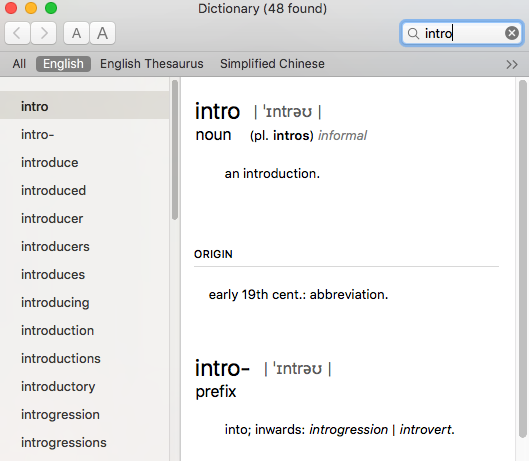
\includegraphics[scale=0.5]{img/edict-en.png}
  \caption{电子词典。所有和用户输入匹配的候选单词全被列出}
  \label{fig:e-dict}
\end{figure}

电子词典通常存有数十万单词。进行全词查找的开销很大。商业电子词典软件会同时使用多重方法以提高性能,包括缓存(caching)、索引(indexing)等等。

和电子词典类似,图\ref{fig:word-completion}显示了某互联网搜索引擎的界面。当用户输入内容后,会列出一些可能的候选搜索项。这些项的开头部分和用户输入相匹配\footnote{实际功能会更加复杂,包括拼写检查,关键词提取、引导等。},并且按照被搜索的热门程度排序。被搜索的次数越多,越排在前面。

\begin{figure}[htbp]
  \centering
  
\includegraphics[scale=0.5]{img/adaptive-input.png}
  \caption{搜索引擎。和用户输入匹配的候选搜索被列出}
  \label{fig:word-completion}
\end{figure}

这两个例子中,软件都提供了某种自动完成的机制。在某些现代的IDE(集成开发环境)中,编辑器还可以帮助用户自动完成程序代码。

我们看看如何使用前缀树来实现电子词典。为了简化问题,假设我们的词典是英—英词典。

词典中保存了key-value对,key是英文单词或者词组,value是对应的解释。

当用户输入‘a’的时候,词典不是只给出‘a’的意思,而是提供一系列候选单词的列表。这些候选单词都以‘a’开头,包括abandon、about、accent、adam……当然,这些都是存储在前缀树中的单词。

如果候选单词太多,一种方案是只显示前10个,如果用户查找的单词不在其中,他可以浏览更多的候选项。如果待查找的字符串为空,我们从当前节点扩展出前$n$个子节点作为候选项;否则,我们递归地在有共同前缀的子分支中查找。

在支持惰性求值(lazy evaluation)的编程环境中,一种简单直观的方法是惰性扩展全部的子节点,然后根据需要取前$n$个。记前缀树前缀树为$T = (v, C)$,下面的函数枚举所有以$k$开头的内容。

\be
findAll(T, k) = \left \{
  \begin{array}
  {r@{\quad:\quad}l}
  enum(C) & k = \phi, v = \phi \\
  \{(\phi, v)\} \cup enum(C) & k = \phi, v \neq \phi \\
  find(C, k) & k \neq \phi
  \end{array}
\right.
\ee

前两行处理key为空的边界情况。此时,我们通过枚举扩展所有数据不为空的子节点。最后一行调用$find$函数寻找和前缀$k$匹配的子分支。

如果节点的子分支不为空,记$C = \{(k_1, T_1), (k_2, T_2), ..., (k_m, T_m)\}$,令除去第一对映射以外的剩余映射为$C'$。枚举算法可以定义如下:

\be
enum(C) = \left \{
  \begin{array}
  {r@{\quad:\quad}l}
  \phi & C = \phi \\
  mapAppend(k_1, findAll(T_1, \phi)) \cup enum(C')
  \end{array}
\right.
\ee

其中$mapAppend(k, L) = \{(k + k_i, v_i)| (k_i, v_i) \in L\}$。它将前缀$k$添加到列表$L$中的所有key-value对的key前面\footnote{可以进一步抽象为对第一个元素进行映射。在Haskell中,使用范畴论中的箭头概念,$mapAppend$可被表示为$map(first(k+), L)$}。

函数$enum$也可用$concatMap$的概念定义(亦称为$flatMap$)\footnote{效果上相当于先对每个元素进行映射,然后将结果连接起来。通常使用build-foldr来消除中间结果中的列表}。

\be
enum(C) = concatMap(\lambda_{(k, T)} . mapAppend(k, findAll(T, \phi)))
\ee

函数$find(C, k)$定义如下。如果子树为空,结果也为空;否则,它首先检查$k_1$映射的子树$T_1$。如果$k_1$和$k$相等,就调用$mapAppend$向$T_1$所有子分支的key前增加前缀$k$;如果$k_1$是$k$的前缀,算法就递归地查找所有以$k - k_1$开头的子分支;反之,如果$k$是$k_1$的前缀,则$T_1$的所有子分支都是候选项。否则,算法跳过第一对映射,继续处理剩余的其他映射。

\be
find(C, k) = \left \{
  \begin{array}
  {r@{\quad:\quad}l}
  \phi & C = \phi \\
  mapAppend(k_1, findAll(T_1, \phi)) & k \sqsubset k_1 \\
  mapAppend(k_1, findAll(T_1, k - k_1)) & k_1 \sqsubset k \\
  find(C', k) & otherwise
  \end{array}
\right.
\ee

下面的Haskell例子程序按照上述算法实现了一个简单的电子词典:

\lstset{language=Haskell}
\begin{lstlisting}[style=Haskell]
import Control.Arrow (first)

get n t k = take n $ findAll t k

findAll :: Eq k => PrefixTree k v -> [k] -> [([k], v)]
findAll (PrefixTree Nothing cs) [] = enum cs
findAll (PrefixTree (Just x) cs) [] = ([], x) : enum cs
findAll (PrefixTree _ cs) k = find' cs k
  where
    find' [] _ = []
    find' ((k', t') : ps) k
          | k `isPrefixOf` k'
              = map (first (k' ++)) (findAll t' [])
          | k' `isPrefixOf` k
              = map (first (k' ++)) (findAll t' $ drop (length k') k)
          | otherwise = find' ps k

enum :: Eq k => [([k], PrefixTree k v)] -> [([k], v)]
enum = concatMap (\(k, t) -> map (first (k ++)) (findAll t []))
\end{lstlisting}

在Haskell这样的惰性求值编程环境中,前$n$个候选项可以通过$take(n, findAll(T, k))$来获取。附录A给出了$take$函数的详细定义。

也可以用命令式的方式实现电子词典。下面的算法复用了前面定义的前缀树查找函数。当我们找到一个节点,其对应的前缀和用户输入的内容一致时,算法将扩展该节点的所有子树直到获取到前$n$个候选项。

\begin{algorithmic}[1]
\Function{Look-Up}{$T, k, n$}
  \If{$T = $ NIL}
     \State \Return $\phi$
  \EndIf
  \State $prefix \gets$ NIL
  \Repeat
    \State $match \gets$ FALSE
    \For{$\forall (k_i, T_i) \in $ \Call{Children}{$T$}}
      \If{$k$ is prefix of $k_i$}
        \State \Return \Call{Expand}{$prefix + k _i, T_i, n$}
      \EndIf
      \If{$k_i$ is prefix of $k$}
        \State $match \gets$ TRUE
        \State $k \gets k - k_i$
        \State $T \gets T_i$
        \State $prefix \gets prefix + k_i$
        \State break
      \EndIf
    \EndFor
  \Until{$\lnot match$}
  \State \Return $\phi$
\EndFunction
\end{algorithmic}

其中函数\textproc{Expand}($T, prefix, n$)选取$n$个子树,这些子树在$T$中有同样的前缀。它的实现为广度优先遍历(BFS),本书最后一章对包括广度优先在内的搜索算法有详细的介绍。

\begin{algorithmic}[1]
\Function{Expand}{$prefix, T, n$}
  \State $R \gets \phi$
  \State $Q \gets \{(prefix, T)\}$
  \While{$|R| < n \land Q$ is not empty}
    \State $(k, T) \gets$ \Call{Pop}{$Q$}
    \If{\Call{Data}{$T$} $\neq$ NIL}
      \State $R \gets R \cup \{(k, $ \Call{Data}{$T$} $)\}$
    \EndIf
    \For{$\forall (k_i, T_i) \in$ \Call{Children}{$T$} in sorted order}
      \State \Call{Push}{$Q, (k + k_i, T_i)$}
    \EndFor
  \EndWhile
\EndFunction
\end{algorithmic}

下面的Python例子程序实现了一个电子词典。它使用了标准库中的\texttt{find}函数来判断一个字符串是否是另一个的前缀。

\lstset{language=Python}
\begin{lstlisting}
def lookup(t, key, n):
    if t is None:
        return []
    prefix = ""
    while True:
        match = False
        for k, tr in t.subtrees.items():
            if string.find(k, key) == 0: # key is prefix of k
                return expand(prefix + k, tr, n)
            if string.find(key, k) ==0:
                match = True
                key = key[len(k):]
                t = tr
                prefix += k
                break
        if not match:
            break
    return []

def expand(prefix, t, n):
    res = []
    q = [(prefix, t)]
    while len(res)<n and q:
        (s, p) = q.pop(0)
        if p.value is not None:
            res.append((s, p.value))
        for k, tr in sorted(p.subtrees.items()):
            q.append((s + k, tr))
    return res
\end{lstlisting}

%=====================================
% T9
%=====================================

\subsection{T9输入法}
\index{T9}
\index{Textonym输入法}

手机用户编辑短信或者电子邮件时的体验和PC上完全不同。手机键盘(称为ITU-T键盘)上只有非常少的按键。如图\ref{fig:itut-keypad}所示。

\begin{figure}[htbp]
  \centering
  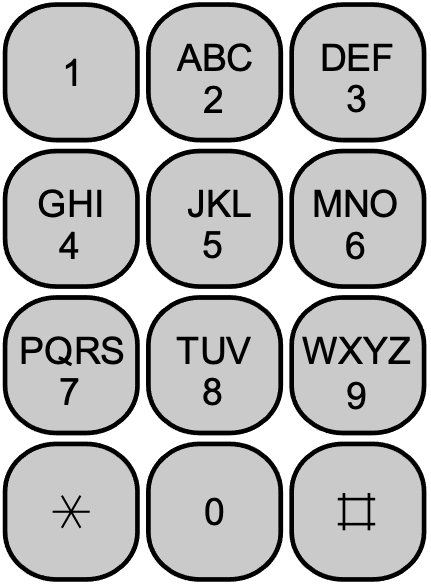
\includegraphics[scale=0.4]{img/itu-t.png}
  \caption{手机ITU-T键盘}
  \label{fig:itut-keypad}
\end{figure}

在ITU-T键盘上输入英文单词或短语有两种方法。例如用户要输入单词home,他需要按照下面的顺序按键:

\begin{itemize}
\item 按两次4键以输入字符h;
\item 按三次6键以输入字符o;
\item 按一次6键以输入字符m;
\item 按两次3键以输入字符e;
\end{itemize}

另外一种更快速的方法使用下面的按键顺序:

\begin{itemize}
\item 依次按下4、6、6、3,单词home出现在候选列表的最上方;
\item 按下‘*’号键以变换不同的候选单词,good此时出现在候选列表上;
\item 按下‘*’号键再次变换,下一个候选单词gone出现在列表上;
\item ……
\end{itemize}

对比这两个方法,可以发现后者更加方便,但是需要额外保存一个候选单词字典。这种方法被称作“T9输入法”或预测输入法\cite{wiki-t9}、\cite {wiki-predictive-text}。T9是英文textonym的缩写,它以T开头,后面跟9个字母。T9输入法可以用前缀树来实现。

为了向用户提供候选单词,T9输入法需要预先准备一个词典。商业上的T9输入法通常使用更加复杂的索引词典,同时在文件系统和缓存中进行快速索引。本节中的实现仅仅出于演示的目的。

首先我们需要定义T9键盘映射,它将数字映射为候选字符。

\be
\begin{array}{ll}
M_{T9} = \{ & 2 \rightarrow abc, 3 \rightarrow def, 4 \rightarrow ghi, \\
           & 5 \rightarrow jkl, 6 \rightarrow mno, 7 \rightarrow pqrs, \\
           & 8 \rightarrow tuv, 9 \rightarrow wxyz \}
\end{array}
\ee

使用这一映射后,$M_{T9}[i]$就返回数字$i$对应的若干个字符。我们也可以定义从字符到数字的逆映射。

\be
M^{-1}_{T9} = concat(\{\{c \rightarrow d | c \in S\} | (d \rightarrow S) \in M_{T9}\})
\ee

通过查找$M^{-1}_{T9}$,我们可以将字符串转换成一组按键序列。

\be
digits(S) = \{ M^{-1}_{T9}[c]| c \in S \}
\ee


给定一个数字序列$D = d_1d_2...d_n$,我们定义T9查找的算法如下。

\be
findT9(T, D) = \left \{
  \begin{array}
  {r@{\quad:\quad}l}
  \{ \phi \} & D = \phi \\
  concatMap(find, prefixes(T)) & otherwise
  \end{array}
\right.
\ee

其中$T$是从一组单词和词组中构造出的前缀树。我们将其作为T9输入法的词典。若输入的数字串$D$为空,则候选单词的结果列表也是空。否则,我们搜索匹配输入的子树并将结果连接起来。

为了枚举所有匹配的子树,我们检查子树集$C_T$中的每一对$(k_i, T_i)$。首先将字符串$k_i$转换为数字串$d_i$,然后比较$d_i$和$D$。如果其中之一是另一个的前缀,则选中这一对$(k_i, T_i)$进行进一步查找。

\be
prefixes(T) = \{(k_i, T_i) | (k_i, T_i) \in C_T, d_i = digits(k_i), d_i \sqsubset D \lor D \sqsubset d_i \}
\ee

函数$find$接受两个参数,一个前缀$S$和需要进一步查找的子树$T'$。其中$S$是$D$的前缀。为此,我们从$D$中去除这一前缀,然后用剩余的数字串$D' = D - S$继续查找。最后再将$S$添加回递归查找的各个结果前面。

\be
find(S, T') = \{ take(n, S + s_i) | s_i \in findT9(T', D - S) \}
\ee

其中$n = |D|$是输入数字串的长度。函数$take(n, L)$从列表$L$中获取前$n$个元素。如果列表的长度短于$n$,则获取全部元素。

下面的Haskell例子程序实现了从前缀树查找的T9输入法。

\lstset{language=Haskell}
\begin{lstlisting}
import qualified Data.Map as Map

mapT9 = Map.fromList [('1', ",."), ('2', "abc"), ('3', "def"), ('4', "ghi"),
                      ('5', "jkl"), ('6', "mno"), ('7', "pqrs"), ('8', "tuv"),
                      ('9', "wxyz")]

rmapT9 = Map.fromList $ concatMap (\(d, s) -> [(c, d) | c <- s]) $ Map.toList mapT9

digits = map (\c -> Map.findWithDefault '#' c rmapT9)

findT9 :: PrefixTree Char v -> String -> [String]
findT9 t [] = [""]
findT9 t k = concatMap find prefixes
  where
    n = length k
    find (s, t') = map (take n . (s++)) $ findT9 t' (k `diff` s)
    diff x y = drop (length y) x
    prefixes = [(s, t') | (s, t') <- children t, let ds = digits s in
                          ds `isPrefixOf` k || k `isPrefixOf` ds]
\end{lstlisting}  %$

可以使用广度优先搜索实现命令式的T9输入法。我们使用一个队列$Q$,其保存的元素为三元组
$(prefix, D, T)$。每个三元组包含一个已搜索过的前缀$prefix$,尚未搜索的剩余部分$D$,
还有待搜索的子树$T$。队列初始的时候,三元组包含一个空前缀,全部待搜索的数字,以及前缀树
的根节点。算法不断从队列中取出三元组,对其中的树$T$,依次检查它的子树$T_i$。通过检索
T9的逆映射,我们将子树对应的前缀串$k_i$转换成数字串$D'$。如果$D$是$D'$的前缀,说明
找到了一个候选单词。我们将$k_i$添加到三元组中的前缀$prefix$后,并纪录下这一结果。
如果$D'$是$D$的前缀,我们需要继续在这棵子树中查找。为此,我们将已$k_i$结尾的前缀,
剩余的数字串$D-D'$和该子树组成一个新的三元组,放入队列的尾部。

\begin{algorithmic}[1]
\Function{Look-Up-T9}{$T, D$}
  \State $R \gets \phi$
  \If{$T =$ NIL or $D = \phi$}
    \State \Return $R$
  \EndIf
  \State $n \gets |D|$
  \State $Q \gets \{(\phi, D, T)\}$
  \While{$Q \neq \phi$}
    \State $(prefix, D, T) \gets$ \Call{Pop}{$Q$}
    \For{$\forall (k_i, T_i) \in $ \Call{Children}{$T$}}
      \State $D' \gets$ \Call{Digits}{$k_i$}
      \If{$D' \sqsubset D$} \Comment{$D'$ is prefix of $D$}
        \State $R \gets R \cup \{$ \textproc{Take} $(n, prefix + k_i) \}$ \Comment{限制长度不超过$n$}
      \ElsIf{$D \sqsubset D'$}
        \State \textproc{Push}($Q, (prefix + k_i, D - D', T_i)$)
      \EndIf
    \EndFor
  \EndWhile
  \State \Return $R$
\EndFunction
\end{algorithmic}

函数\textproc{Digits}($S$)将字符串$S$转换为数字串。

\begin{algorithmic}[1]
\Function{Digits}{$S$}
  \State $D \gets \phi$
  \For{each $c \in S$}
    \State $D \gets D \cup \{M^{-1}_{T9}[c]\}$
  \EndFor
  \State \Return $D$
\EndFunction
\end{algorithmic}

下面的Python例子程序使用前缀树实现了T9输入法。

\lstset{language=Python}
\begin{lstlisting}
T9MAP={'2':"abc", '3':"def", '4':"ghi", '5':"jkl", \
       '6':"mno", '7':"pqrs", '8':"tuv", '9':"wxyz"}

T9RMAP = dict([(c, d) for d, cs in T9MAP.items() for c in cs])

def digits(w):
    return ''.join([T9RMAP[c] for c in w])

def lookup_t9(t, key):
    if t is None or key == "":
        return []
    res = []
    n = len(key)
    q = [("", key, t)]
    while q:
        prefix, key, t = q.pop(0)
        for k, tr in t.subtrees.items():
            ds = digits(k)
            if string.find(ds, key) == 0: # key is prefix of ds
                res.append((prefix + k)[:n])
            elif string.find(key, ds) == 0: # ds is prefix of key
                q.append((prefix + k, key[len(k):], tr))
    return res
\end{lstlisting}

\begin{Exercise}
\begin{itemize}
\item 使用Trie实现电子词典和T9输入法。
\item 对于返回多个候选结果的前缀树查找算法,如何保证输出的结果按照字典顺序排序?这会对性能产生怎样的影响?
\item 如果不使用惰性求值,如何实现函数式的电子词典和T9输入法?
\end{itemize}
\end{Exercise}

% ================================================================
%                 Short summary
% ================================================================
\section{小结}

本章一开始介绍了整数Trie和前缀树。基于整数前缀树的映射结构在编译器的实现中得到了重要的应用。字符Trie和字符前缀树可以看做是整数映射结构的自然扩展。它们可以被用来处理文字信息。作为例子,我们介绍了自动预测完成输入的电子词典和T9输入法。尽管和商业软件的实现不同,这些例子展示了如何使用Trie和前缀树来解决问题的方法。某些重要的数据结构,如后缀树和本章中介绍的内容紧密相关。读者可以参考附录D。

\ifx\wholebook\relax\else
\begin{thebibliography}{99}

\bibitem{CLRS}
Thomas H. Cormen, Charles E. Leiserson, Ronald L. Rivest and Clifford Stein.
``Introduction to Algorithms, Second Edition''. Problem 12-1. ISBN:0262032937. The MIT Press. 2001(《算法导论》)

\bibitem{okasaki-int-map}
Chris Okasaki and Andrew Gill. ``Fast Mergeable Integer Maps''. Workshop on ML, September 1998, pages 77-86.  \url{http://www.cse.ogi.edu/~andy/pub/finite.htm}

\bibitem{patricia-morrison}
D.R. Morrison, ``PATRICIA -- Practical Algorithm To Retrieve  Information Coded In Alphanumeric", Journal of the ACM, 15(4), October 1968, pages 514-534.

\bibitem{wiki-suffix-tree}
Suffix Tree, Wikipedia. \url{http://en.wikipedia.org/wiki/Suffix_tree}

\bibitem{wiki-trie}
Trie, Wikipedia. \url{http://en.wikipedia.org/wiki/Trie}

\bibitem{wiki-t9}
T9 (predictive text), Wikipedia. \url{http://en.wikipedia.org/wiki/T9_(predictive_text)}

\bibitem{wiki-predictive-text}
Predictive text,
Wikipedia. \url{http://en.wikipedia.org/wiki/Predictive_text}

\end{thebibliography}

\end{document}
\fi
